\documentclass[tikz,border=2pt]{standalone}
\usepackage[T1]{fontenc}
\usepackage{helvet}
\renewcommand{\familydefault}{\sfdefault}
\usetikzlibrary{positioning,arrows.meta,calc}
\definecolor{navy}{HTML}{011E4B}
\definecolor{gold}{HTML}{FAB001}
\definecolor{sky}{HTML}{87C6E9}
\definecolor{alert}{HTML}{EE1C23}

\tikzset{
  >={Stealth[length=2.2mm,width=1.7mm]},
  panel/.style={draw=navy, line width=0.6pt, fill=white, rounded corners=2pt, anchor=north west},
  op/.style={draw=navy, line width=0.6pt, fill=white, rounded corners=2pt, align=center,
             font=\scriptsize\color{navy}, minimum height=9mm, minimum width=2.75cm, inner sep=2pt},
  pill/.style={fill=navy, text=white, rounded corners=4.5mm, align=center, font=\scriptsize\bfseries,
               minimum height=9mm, minimum width=2.75cm, inner sep=3pt},
  goldpill/.style={fill=gold, text=navy, rounded corners=4.5mm, align=center, font=\scriptsize\bfseries,
               minimum height=9mm, minimum width=1.9cm, inner sep=3pt},
  store/.style={draw=navy, line width=0.6pt, fill=white, align=center, font=\scriptsize\color{navy},
               minimum height=9mm, minimum width=2.75cm, inner sep=2pt, double, double distance=1pt},
  advbox/.style={draw=alert, line width=0.8pt, fill=white, rounded corners=2pt, align=center,
             font=\scriptsize\color{navy}, minimum height=9mm, minimum width=2.75cm, inner sep=2pt},
  flow/.style={->, draw=navy, line width=0.9pt},
  sflow/.style={->, draw=sky, line width=1.8pt},
  aflow/.style={->, draw=alert, line width=0.9pt, densely dashed},
  kflow/.style={->, draw=navy, line width=0.7pt, densely dotted},
  ptitle/.style={font=\footnotesize\bfseries\color{navy}, anchor=north west, inner sep=0pt},
  pcap/.style={font=\scriptsize\itshape\color{navy}, anchor=north west, inner sep=0pt},
  lbl/.style={font=\scriptsize\bfseries\color{navy}, fill=white, inner sep=1pt},
  tier/.style={circle, fill=gold, text=navy, font=\scriptsize\bfseries, inner sep=0pt, minimum size=4.4mm},
}
% panel with a solid side tab: #1 name, #2 x, #3 y (top-left), #4 width, #5 height, #6 tab colour
\newcommand{\tabpanel}[6]{%
  \node[panel, minimum width=#4, minimum height=#5] (#1) at (#2,#3) {};
  \fill[#6] ($(#1.north west)+(0.02,-0.02)$) rectangle ($(#1.south west)+(0.17,0.02)$);}

\begin{document}
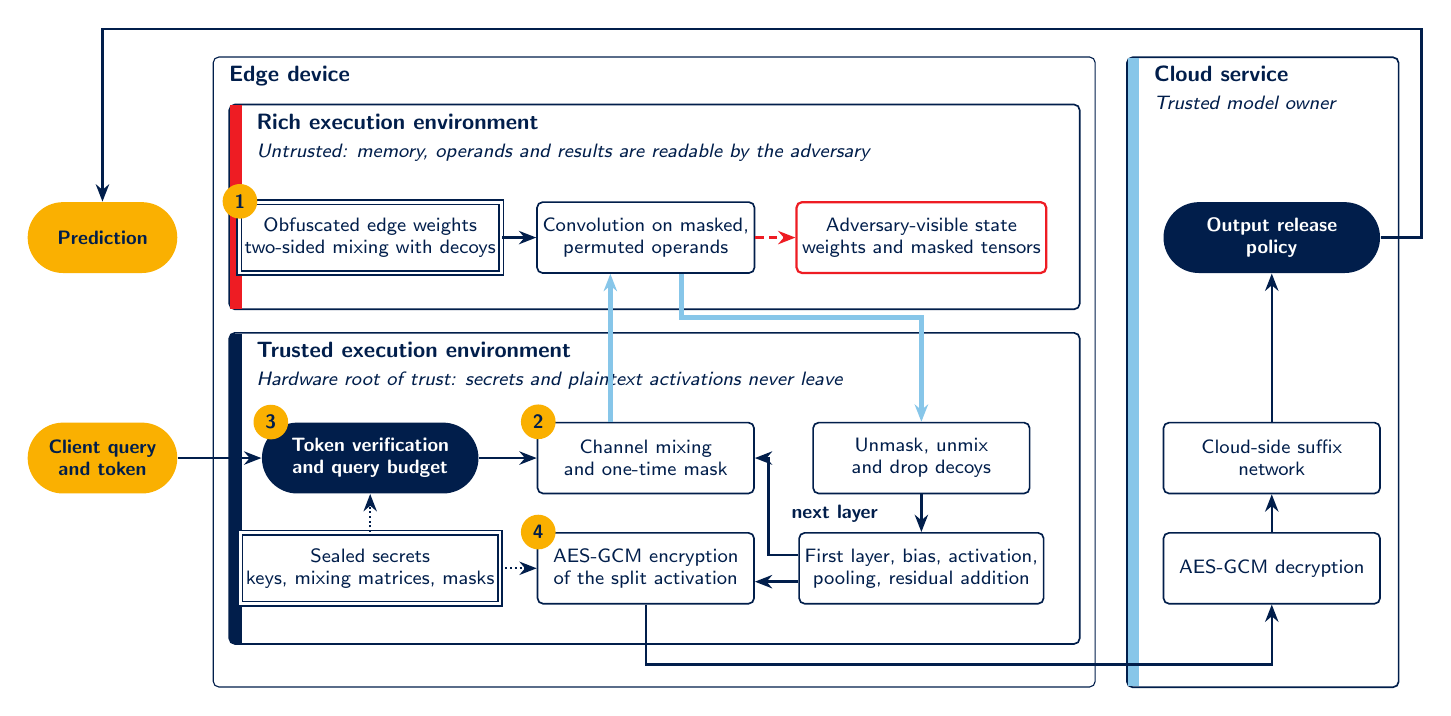
\begin{tikzpicture}
% columns (centres) and rows
\def\cA{4.55} \def\cB{8.05} \def\cC{11.55}
\def\rR{-1.75}            % REE row
\def\rT{-4.55} \def\rU{-5.95}   % TEE rows

% ------------------------------------------------------------ edge device frame
\node[panel, minimum width=11.2cm, minimum height=8.0cm, line width=0.4pt] (dev) at (2.55,0.55) {};
\node[ptitle] at (2.75,0.43) {Edge device};

\tabpanel{ree}{2.75}{-0.05}{10.8cm}{2.6cm}{alert}
\node[ptitle] at (3.1,-0.17) {Rich execution environment};
\node[pcap]   at (3.1,-0.55) {Untrusted: memory, operands and results are readable by the adversary};

\tabpanel{tee}{2.75}{-2.95}{10.8cm}{3.95cm}{navy}
\node[ptitle] at (3.1,-3.07) {Trusted execution environment};
\node[pcap]   at (3.1,-3.45) {Hardware root of trust: secrets and plaintext activations never leave};

% REE row
\node[store]  (wstore) at (\cA,\rR) {Obfuscated edge weights\\two-sided mixing with decoys};
\node[op]     (conv)   at (\cB,\rR) {Convolution on masked,\\permuted operands};
\node[advbox] (adv)    at (\cC,\rR) {Adversary-visible state\\weights and masked tensors};
\draw[flow]  (wstore) -- (conv);
\draw[aflow] (conv) -- (adv);

% TEE rows
\node[pill]  (gate)    at (\cA,\rT) {Token verification\\and query budget};
\node[op]    (mask)    at (\cB,\rT) {Channel mixing\\and one-time mask};
\node[op]    (unmask)  at (\cC,\rT) {Unmask, unmix\\and drop decoys};
\node[store] (secrets) at (\cA,\rU) {Sealed secrets\\keys, mixing matrices, masks};
\node[op]    (aes)     at (\cB,\rU) {AES-GCM encryption\\of the split activation};
\node[op]    (nonlin)  at (\cC,\rU) {First layer, bias, activation,\\pooling, residual addition};

\draw[flow]  (gate) -- (mask);
\draw[sflow] ($(mask.north)+(-0.45,0)$) -- ($(conv.south)+(-0.45,0)$);
\draw[sflow] ($(conv.south)+(0.45,0)$) -- ++(0,-0.55) -| (unmask.north);
\draw[flow]  (unmask) -- (nonlin);
\draw[flow]  ($(nonlin.west)+(0,0.17)$) -- ++(-0.38,0) |- (mask.east);
\node[lbl, anchor=west] at (9.86,-5.25) {next layer};
\draw[flow]  ($(nonlin.west)+(0,-0.17)$) -- ($(aes.east)+(0,-0.17)$);
\draw[kflow] (secrets) -- (gate);
\draw[kflow] (secrets.east) -- ($(aes.west)$);

% ------------------------------------------------------------ cloud
\tabpanel{cloud}{14.15}{0.55}{3.45cm}{8.0cm}{sky}
\node[ptitle] at (14.5,0.43) {Cloud service};
\node[pcap]   at (14.5,0.05) {Trusted model owner};
\node[op, minimum width=2.75cm] (dec)    at (16.0,\rU) {AES-GCM decryption};
\node[op, minimum width=2.75cm] (suffix) at (16.0,\rT) {Cloud-side suffix\\network};
\node[pill, minimum width=2.75cm] (policy) at (16.0,\rR) {Output release\\policy};
\draw[flow] (aes.south) -- (\cB,-7.17) -| (dec.south);
\draw[flow] (dec) -- (suffix);
\draw[flow] (suffix) -- (policy);

% ------------------------------------------------------------ client
\node[goldpill] (client) at (1.15,\rT) {Client query\\and token};
\node[goldpill] (pred)   at (1.15,\rR) {Prediction};
\draw[flow] (client) -- (gate);
\draw[flow] (policy.east) -- (17.9,\rR) -- (17.9,0.9) -| (pred.north);

% ------------------------------------------------------------ tier badges
\node[tier] at ($(wstore.north west)+(0.02,0)$) {1};
\node[tier] at ($(mask.north west)+(0.02,0)$) {2};
\node[tier] at ($(gate.north west)+(0.12,0)$) {3};
\node[tier] at ($(aes.north west)+(0.02,0)$) {4};
\end{tikzpicture}
\end{document}
